
\chapter{基于GPU并行计算的搜索速度优化}
\label{chap:gpu}

本章节中我们将着重介绍我们针对Kaldi开源工具包的一个扩展,以便使它能够支持图形处理芯片(GPU)上的WFST解码推理。该框架可以显著加速现有推理算法,特别是在基于深度序列学习的一系列模型上进行了验证。

我们将维特比算法中的令牌合并操作实现为一个GPU并行计算中的原子操作,以便减少维特比束剪枝算法中同步消耗;我们提出了动态负载均衡的方式以更高效地进行并行计算,提高其多线程之间的利用率;我们重新设计了基于GPU并行计算的精确的词图生成和剪枝算法,以便充分利用GPU的性能特点。

在Switchboard 上实验表明,我们所提出的方法在取得完全一致的1-best和词图质量情况下,可以得到3-15倍的加速,并在绝大部分GPU架构上进行了验证。除此之外,如果再进行多句子的并行处理,最终的加速比将达到46倍。


\section{引言}
\label{chap:gpu-intro}

近来深度学习语音识别的发展唤起了大量语音识别转录的需求。在这一系统中,计算量较大的部分主要包括:声学模型推理和语言模型WFST解码。

为了减少声学模型推理的计算消耗,研究人员们提出了一系列效率更高的声学模型,包括一些比较新颖的神经网络结构~\cite{xue2014singular,peddinti2018low}, 定点化
~\cite{mcgraw2016personalized}, 跳帧~\cite{pundak2016lower,zhc00-chen-is16,zhc00-chen-tasl2017}
和端到端系统~\cite{audhkhasi2017direct,e2e-2018}.
%frame sub-sample or PSD, novel model, SVD, quantization, ...
同时算法的改进,比如剪枝~\cite{mohri2002weighted,hori2004fast}
和向前预测~\cite{soltau2009dynamic,nolden2012search}是针对解码部分主要的加速方式。
%in WFST framework, pruning , lookahead ... in e2e framework...

基于GPU的并行计算是另一种潜在的针对语音识别计算的加速方式。针对声学模型推理,由于大部分计算量集中在矩阵形式的运算,因此它易于通过将类似于训练过程中\cite{vesely2010parallel}的序列批处理~\cite{dixon2009harnessing} 引入推理阶段,以加速运算。
但是,基于GPU并行计算的WFST解码并不容易实现。尽管一些研究在小型语言模型上取得了一定成功~\cite{you2009parallel},但这些系统仍然受制于两部分缺陷:i) 由于GPU显存有限,这些方法并不能有效利用较大的商用语言模型。
ii) 这些方法并不通用,常常受制于特定的声学或语言模型,并且没有词图生成功能。 %Detailed comparisons are in
%Section~\ref{sec:relate}. 
%is another ... , show  potential to allow  speech processing ...  and can be applied on all above model or algorithm side trials.
%to speedup the first part.  batching
% second part insufficient, 
%especially in the context of deep Learning, 
%lack of lattice processing; 
%hard to utilize large LM
%


这项工作作为Kaldi工具包的一个扩展~\cite{povey2011kaldi},实现了基于GPU并行计算的WFST解码。
%
这是一个通用的离线解码器~\footnote{近期的研究显示,使用CPU比较容易得到一个实时的解码器来针对在线解码应用
 ~\cite{peddinti2018low,zhc00-chen-tasl2017} 。因此我们的目标集中在如何解码海量的离线语音,降低其计算损耗。},
 该解码器对语言模型和声学模型没有特别的限制,并且可以工作在各种架构的GPU上。
%
为了支持第二遍重打分和更丰富的后处理,我们的设计基于WFST解码和词图生成的架构~\cite{povey2012generating}。
%
我们对这项工作进行了开源~\footnote{\url{https://github.com/chenzhehuai/kaldi/tree/gpu-decoder}},
它将会与大多数Kaldi脚本相兼容。


\section{维特比算法并行化框架}
\label{chap:gpu-viterbi}

我们所提出的系统工作在二遍解码框架下~\cite{woodland19951994},以便能够支持更大的语言模型,并支持词图上丰富的后处理。

\subsection{系统框架}
\begin{figure*}[ht]
  \centering
    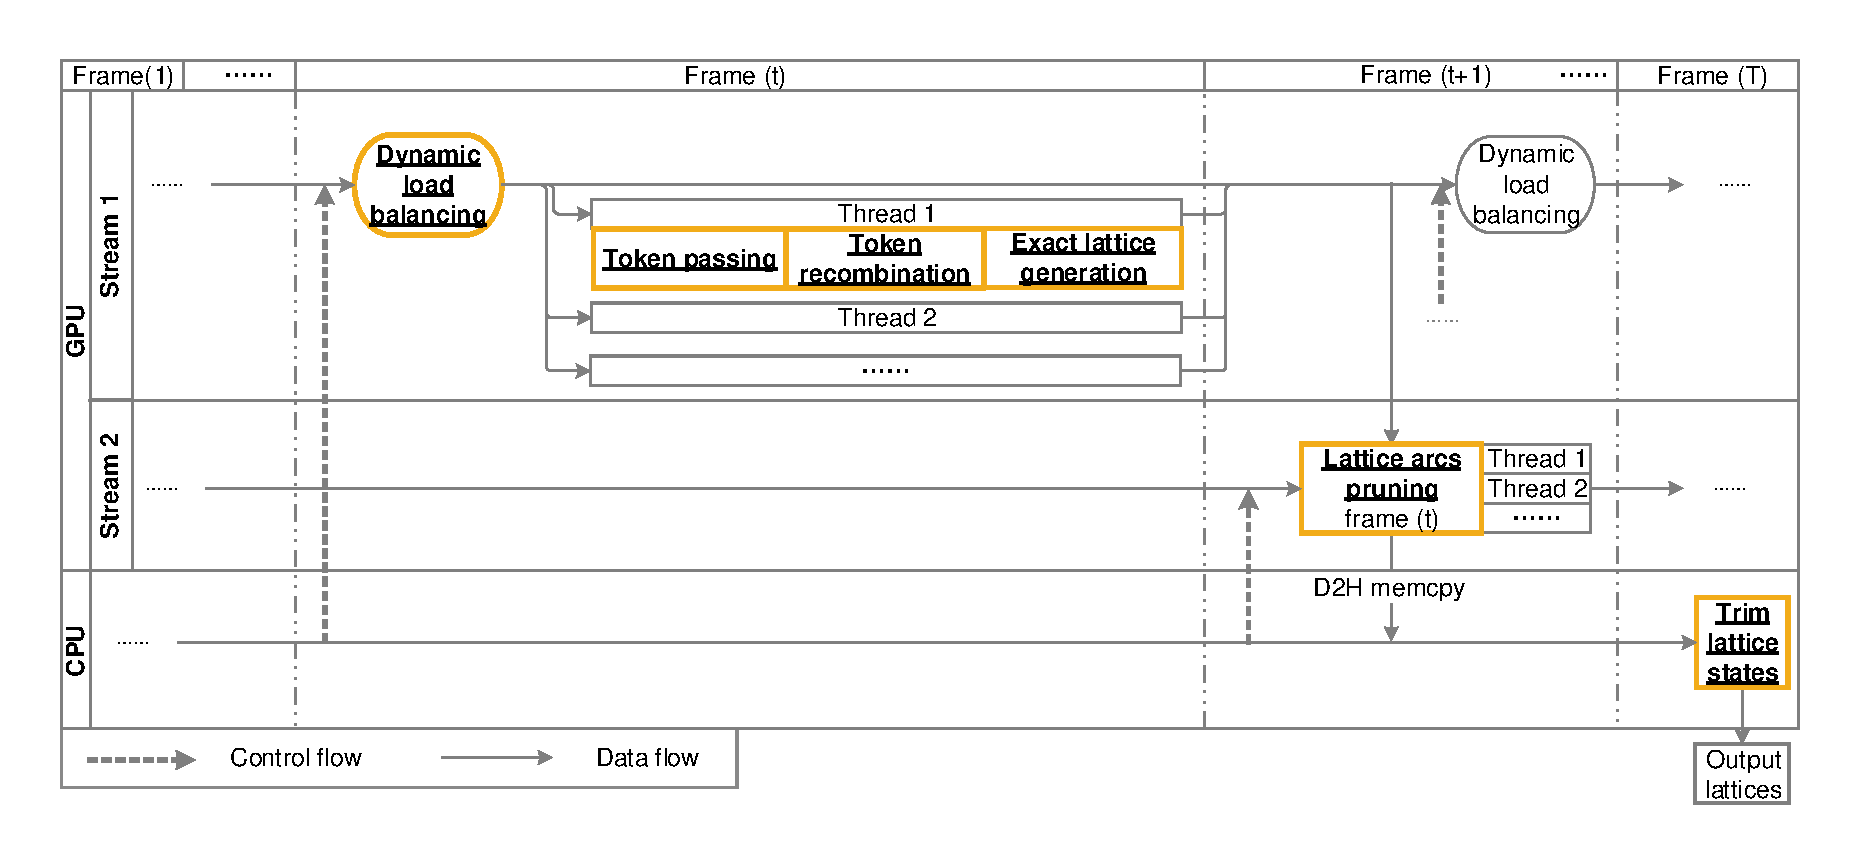
\includegraphics[width=1\linewidth]{figure/gpu_framework.pdf}
    \caption{\it  并行维特比束剪枝算法以及精确词图处理系统的框架}
    \label{fig:gpu-framework}
\end{figure*}
图~\ref{fig:gpu-framework} 显示了系统的框架,这包括两个GPU同时处理流,分别进行解码和词图剪枝,它们完全并行同时受不同CPU线程所控制。具体来说,对第 ($t+1$)帧, 第二个处理流将处理第一个流产生的第($t$)帧的词图。
%GPU and CPU work asynchronously and there are two GPU concurrent streams
%performing decoding and lattice processing respectively.

解码的流程类似于CPU 版本~\cite{povey2011kaldi},但工作在不同的一些设计上,以适应并行计算需求,其罗列于下面的章节。负载均衡算法则处理了线程之间并行的分配,它们具体体现在如何分配WFST状态和边。
%position of 4 topics below in the system and acts like an overall procedure/algorithm




\section{并行的令牌传递算法}
\label{sec:atomic}

下面我们首先介绍维特比搜索中将会引入的同步时间消耗,它具体出现在令牌合并过程中。
%
% Take Hidden Markov Model (HMM) as an example.  It is defined
% as the conditional likelihood $p(\mathbf{O}|\mathbf{L})$ of a feature sequence ${\mathbf O}$ given a label sequence $\mathbf L$.
% \vspace{-2em}
% \begin{eqnarray}
% \label{equ:hmm-model}
% %\begin{split}
% p(\mathbf{O}|\mathbf{L})
% %&=&\!\!\!\!\!\!\sum_{\mathbf{q}\in\mathcal{A}(\mathbf{L})}\!\!\!p(\mathbf{O},\mathbf{q}|{\mathbf L}) =\sum_{\mathbf{q}}\prod_{t=1}^{T} p({\bf o}_{t}|q_t) P(q_t|q_{t-1})\nonumber\\
% %y_{ut}(s^{(r)}_{ut})
% &\propto&\sum_{\mathbf{q} \in\mathcal{A}(\mathbf{L})}\prod_{t=1}^{T} \frac{P(q_t|{\bf o}_{t})}{P(q_t)}P(q_t|q_{t-1})\\
% %\end{split}
% \label{equ:hmm-model-viterbi}
% &\propto&\max_{\mathbf{q}}\prod_{t=1}^{T} \frac{P(q_t|{\bf o}_{t})}{P(q_t)}P(q_t|q_{t-1})
% \end{eqnarray}
% %\end{split}
% where $\mathbf{L}$ is a label sequence, and
% $\mathbf{q}$ is a HMM state sequence and  $q_t$ is the HMM state at frame $t$. $P(q_t|q_{t-1})$ is the HMM state transition probability and $P(q_t)$ is the state prior probability of $q_t$.  The posteriors $P(q_t|{\bf o}_{t})$ are estimated using neural networks (HMM-DNN).
% $\mathcal{A}$ is a mapping function from  $\mathbf{L}$ to its corresponding HMM
% state sequence $\mathbf{q}$. In Viterbi algorithm, the sum over $\mathbf{q}$ in
% Equation~\eqref{equ:hmm-model} is replaced by the best state sequence as shown
% in Equation~\eqref{equ:hmm-model-viterbi}.
%
% An alternative formulation of the Viterbi algorithm is used in ASR, called Token Passing algorithm~\cite{woodland19951994}.
% %
在ASR解码中,维特比搜索被实现为 \textit{令牌传递算法}~\cite{woodland19951994}, 其令牌表示的是截止 $t$帧情况下的一个局部识别序列,同时对于每一个 WFST状态在 $t$帧时都可以用一个可移动的令牌进行表示。
在每一帧,维特比路径是通过 \textit{令牌合并}过程得到的, 其他一个 \textit{min} 操作被加到了每个状态的所有输入边上 (比如对状态7,在图~\ref{fig:load-balance} 中,那么它的输入边包括2至7,5至7,7至7三条), 这里我们需要计算得到它们之中的最佳分数,以及这个分数来自哪一个状态。

%Thus for a state, tokens coming from different paths need to be compared and recombined together in serial. 
%Only the best one is passed to the next WFST state,
%and describe in CPU how to do it.
%
%and it is the bottleneck of parallel methods. 


\begin{algorithm}[ht]
%\vspace{-0.25em}
\caption{线程级别的令牌合并算法 \textcolor[rgb]{0,0.5,0}{(Inputs: accumulated cost, an out-going WFST arc and a current token)}}
\label{code:atomic}
\begin{algorithmic}[1]
\Procedure{Recombine} {cost, arc, curTok}
\State oldTokPack = state2tokPack[arc.next\_state]
\State curTokPack = \textit{packFunc}(cost,arc.id) \Comment \textcolor[rgb]{0,0.5,0}{pack into uint64}
\State ret = \textit{atomicMin}~\footnotemark(oldTokPack,curTokPack)
\If { ret $>$ curTokPack }         \Comment \textcolor[rgb]{0,0.5,0}{recombine}
\State  perArcTokBuf[arc.id] = *curTok \Comment \textcolor[rgb]{0,0.5,0}{store token}
%\State  modified[arcId] = 1
\EndIf
\EndProcedure
%\\
%\textcolor[rgb]{0,0,0}{[A grid barrier before the next procedure]}
%\Procedure{Tok. Storage} {curTokPack, toToken}
%\State arc = \text{unpackFunc}(curTokPack).arc  \Comment \textcolor[rgb]{0.8,0,0}{ back to int32}
%\State *toToken = *perArcTokBuf[arc] \Comment \textcolor[rgb]{0.8,0,0}{recombine stage 2}
%\EndProcedure
\end{algorithmic}
\end{algorithm}
\footnotetext{\textit{atomicMin}({\em{*address}}, {\em{val}})~\cite{cuda9}. Computes \textit{min}({\em{*address}}, {\em{val}}), writes the result to {\em{address}}, and returns the original {\em{*address}} .}

%\textit{atomicMin}(address, val). Read the 64-bit {\em{old}} located at the {\em{address}}, computes the \textit{min} of {\em{old}} and {\em{val}}, and stores the result to {\em{address}}~\cite{cuda9}.}
%\vspace{-1em}

原始的CPU算法在进行令牌合并时候是串行的。我们即将讨论如何在GPU中实现令牌合并,而将如何高效并行这些指令放在下面的章节中。一种最简单的实现是通过添加critical sections~\cite{lamport1979make}
以便使令牌合并这一步仍然恢复串行。这种设计不仅低效,而且会在早期GPU中引入死锁。
\cite{you2009parallel} 提出一种在每个状态上做针对所有令牌传递结果的规约操作,但这样将引入额外的规约过程中的写冲突和同步损耗,而且这些损耗总是发生在计算的最后阶段。
%
\cite{kim2011h} 提出将所有数据编码到32比特上,然后使用GPU原子操作来实现令牌合并。这种方法损失了计算精度,并且使解码算法受制于特定的模型。

我们提出算法~\ref{code:atomic}, 它是一个通用的计算方法,适应于任何模型的令牌合并,没有精度损失。这个算法执行于每一个GPU线程上,并且针对每一条WFST边进行并行,比如在图\ref{fig:load-balance} 中从状态2到状态7的边可以由这一算法进行处理。
% describes the 2-stage atomic operation based token recombination. 
我们首先将分数和边的索引合并为一个64比特整形数,以表示合并之前的令牌, 同时我们将分数放在高位上,使得它可以控制后续的合并结果。在每一帧,我们将所有令牌的信息保存在一个长度为所有可行边的数组上。这保重合并过程没有写入的冲突,也就不会带来同步损耗。领过所有的令牌处理后,我们收集所有仍然活跃的合并令牌,将64比特数字返回原先的分数和边的索引,由此将真正的令牌信息存入相应的令牌中,而这一步也同样是并行进行的。


\section{图搜索的动态负载均衡算法}
\label{sec:para-viterbi}

另一个并行算法的问题是负载均衡。
对每一个状态,我们并行地遍历所有它的输出边,直到到达了一个终止节点。由于WFST状态可能具有完全不同的输出边数,如果不能合理地将线程分配给这些边,将导致负载不均问题。
不同于\cite{you2009parallel,mendis2016parallelizing},这里作者重新设计了 WFST结构以减少这种不均;在这项工作中,我们不希望解码算法依赖于特定的声学,词典,语言模型。
我们首先提出\textit{静态负载均衡算法}, 它首先对每个线程计算如何分配WFST边才能得到大致相等的数量,经过那之后才开始进行处理。这样的设计引入了额外的并行求取累积和的消耗~\footnote{具体来说是一个GPU上的DeviceScan操作,其工作在大约 10K 个整形数上。},
这种方法将引入计算和GPU内核启动的时间消耗。

受~\cite{alakeel2010}的启发,我们进一步引入了
\textit{动态负载均衡算法},其呈现在算法~\ref{code:load-balance}中。我们使用一个调度中心来分配令牌,同时我们令 $N$个线程为一个组 ($N = 32$) 来共同处理从一个状态出发的所有WFST边。当一个令牌的所有边都被处理完毕了,它就会找调度中心取到下一个令牌。我们同事将调度中心实现为一个GPU原子操作。图~\ref{fig:load-balance}显示了其中的一个例子。在实验中我们比较了两种不同的负载均衡算法。


%Algorithm~\ref{code:load-balance} shows dynamic load balancing
\vspace{-0.5em}
\begin{algorithm}[ht]
%\vspace{-0.25em}
\caption{Grid级别的令牌传递算法 \textcolor[rgb]{0,0.5,0}{(N=32; Inputs: the current active token vector)}}
\label{code:load-balance}
\begin{algorithmic}[1]
\Procedure{ Dynamic Load Balancing } {toks}
\State group = cooperative\_groups::tiled\_partition$\left<32\right>$
\If{group.thread\_rank()==0}\Comment\textcolor[rgb]{0,0.5,0}{rank 0 in each group}
\State i = \textit{atomicAdd}(global\_d,1)  \Comment\textcolor[rgb]{0,0.5,0}{allocate new tokens}
\EndIf      %\Comment\textcolor[rgb]{0,0,0}{i=global\_d++}
\State i = group.\textit{shfl}(i,0) \Comment \textcolor[rgb]{0,0.5,0}{rank 0 broadcasts i to whole group}
\If {i$>=$sizeof(toks)} return\Comment \textcolor[rgb]{0,0.5,0}{all tokens processed}
\EndIf 
\For {arc in tok2arcs(toks[i])} \Comment \textcolor[rgb]{0,0.5,0}{thread parallelism}
\State {\bf call} \textit{Recombine}(toks[i].cost+arc.cost, arc, toks[i])
\EndFor
\EndProcedure
\end{algorithmic}
\end{algorithm}


\begin{figure}[ht]
  \centering
    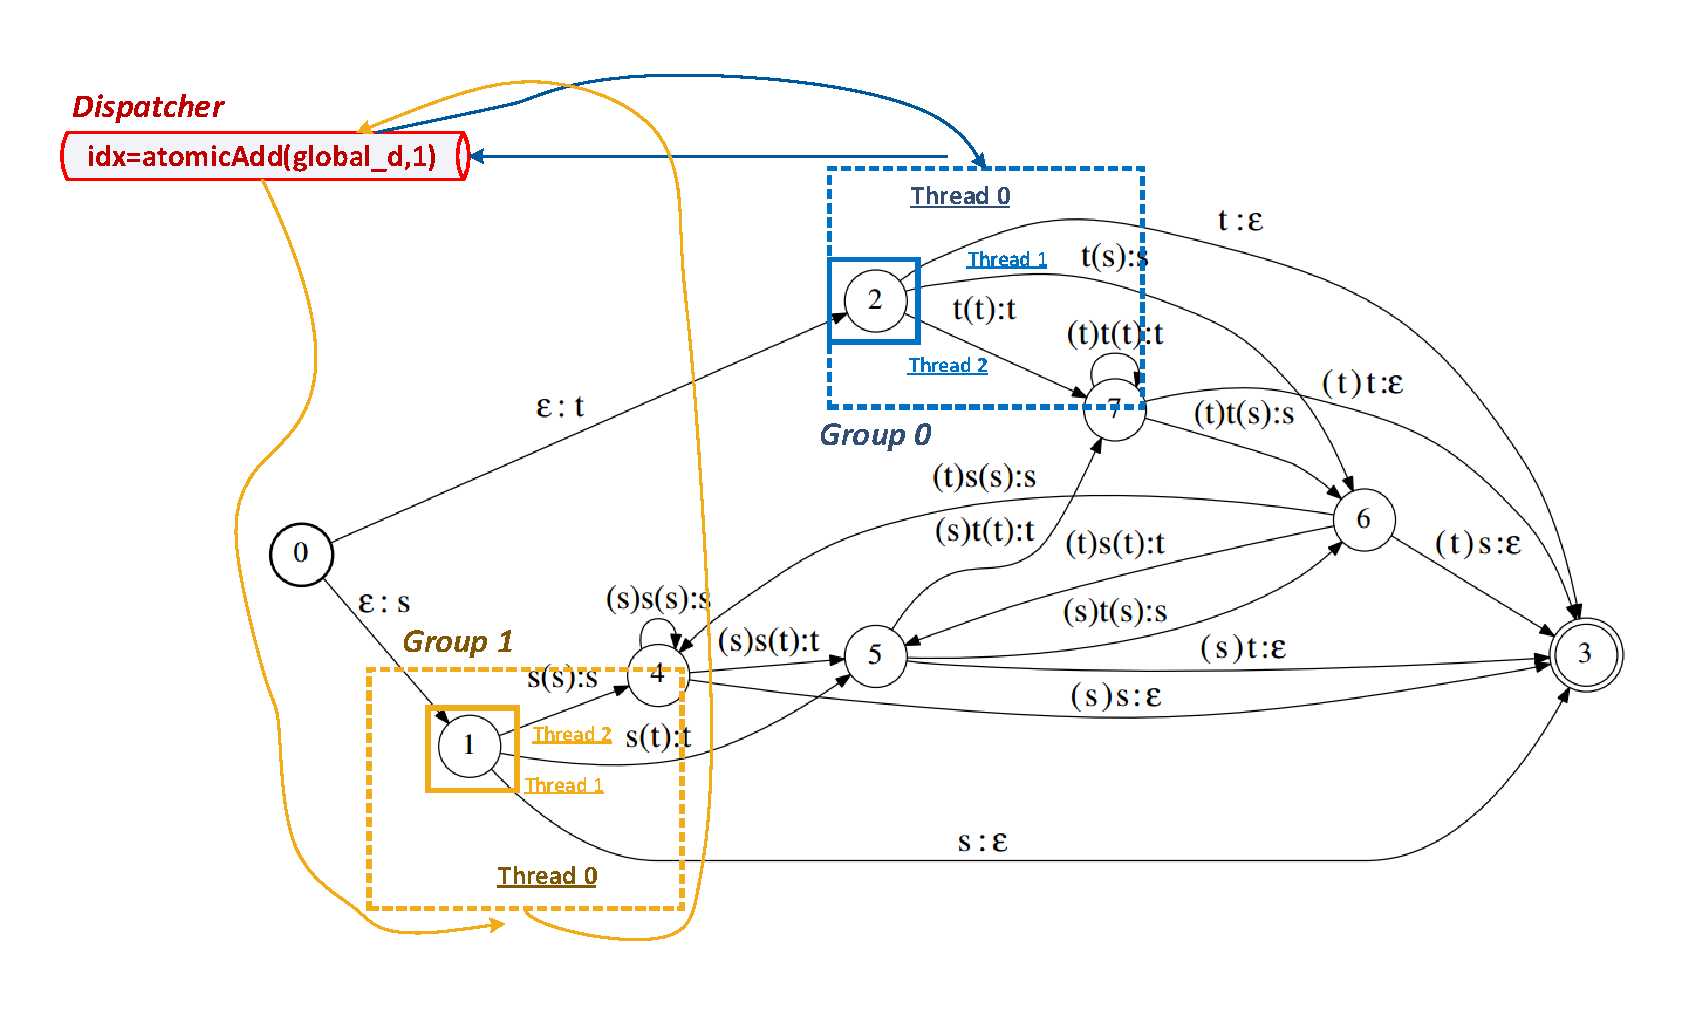
\includegraphics[width=1.1\linewidth]{figure/load-balance.pdf}
    \caption{\it 一个针对动态负载均衡的例子。这里的虚线框表示一个
      CUDA cooperative group ,不同的组分表示为不同的颜色。每一个组由线程0进行控制。当某个组分处理完了从一个状态出发的所有边,线程0将会向调度中心索要下一个令牌,并通知组分里的其他线程。而调度中心使用原子操作来保证每个令牌只分配给一个组分。组0和组1完全工作在并行方式中。}
    \label{fig:load-balance}
\end{figure}

\section{并行的词图处理算法}
\label{sec:lat-gen}


\subsection{精确的词图生成算法}
WFST精确词图~\cite{povey2012generating} 是指在词图上保存了准确的分数和状态级对齐关系,这些信息对于语言模型重打分,丰富的语音识别后处理等都有重要作用。~\footnote{除了本文中研究的置信度应用~\cite{mangu1999finding} ,它同样可以用于加速鉴别性解码~\cite{goel2000minimum},
系统融合~\cite{fiscus1997post}, 鉴别性训练~\cite{povey2005discriminative}, 等等。 .}. %We examine lattice rescoring and confidence measure in this paper.
但是在GPU中实现词图处理算法并不简单。
\cite{kim2014accelerating} 提出在GPU中解码,而后在CPU中生成词图,这不仅使解码器速度下降,而且引入了大量的device-to-host (D2H) 内存拷贝问题。
%(much slower, sec 2.2, fig 2).
我们通过重新设计了一个并行版本的词图处理算法\cite{povey2012generating}更彻底地解决了这个问题。

%enable GPU decoder with large scale LM rescoring (enable GPU decoding in real application).
%ours comparable to no-lat; 

在词图生成中,对每一个令牌传递操作,会有一条词图边被记录到GPU显存中。我们设计了一种GPU向量结构来保存这些边。这种向量实现了  {\em{push\_back}} 算法,其通过原子操作来分配特定内存给相应词图边,而整体内存则被预先分配完毕,增量扩展。

为了较少原子操作所带来的损耗,我们提前分配好 $K$个向量,并随机选取一个向量执行 {\em{push\_back}} 操作。经过令牌传递之后,这些来自$K$ 个向量的边被收集起来。对于词图节点,我们可以使用类似的方案~\footnote{在我们早前的实现中,这一优化可以10倍加速词图边处理的速度,在 $K=32$时。这项加速针对词图节点并不明显。}。



\subsection{词图剪枝}

并行词图剪枝算法基于引文~\cite{ljolje1999efficient,povey2012generating}中方法,并针对GPU并行处理进行了必要的修改。

原始的CPU版本词图剪枝算法会迭代地更新节点和边的额外权重,直到它们停止改变;而额外权重定义为当前边的最佳权重与最佳路径上的权重的差值。对于一些权重过高的边,将会被剪枝,直到一个节点上的所有边都被剪枝。在GPU版本实现中:i) 我们将迭代更新节点和边的过程进行了GPU线程的并行化;
ii) 我们使用一个全局的边向量数组来代替原始实现中的链表结构,原因是链表结构并不能被随意访问(random access),而是总要从头进行访问;
iii) 我们将额外权重迭代更新实现为一个原子操作,以减小同步时间消耗。

 当一条词图边被剪枝后,我们不会物理上删除这条边,原因是内存分配时间消耗较大。相反,我们在剪枝的最后进行并行收集操作,将所有剩余边一次集中到GPU向量结构中,类似于第~\ref{sec:lat-gen}章中的做法。 这种实现方法的内存消耗将会在实验中进行讨论。
%Lattice nodes not associated with remaining arcs are removed in CPU processing for ease of implementation without adding much overhead.
同时,我们没有裁剪词图的节点,原因是:i) 我们需要词图边上能够寻迹到词图节点上,并且在D2H拷贝前后都要有唯一对应,因此我们没有改变节点的相对位置。ii) 在CPU中会重新建立起节点和边的链表关系,因此没有边连接的节点将被隐含删除。 iii)  节点的D2H拷贝是与解码和词图处理异步的,因此不会对最终速度造成影响。

本文提出的词图处理算法总结如下:
 \vspace{-0.25em}
 \begin{algorithm}[ht]
 %\vspace{-0.25em}
 \caption{Grid级别的词图处理算法  \textcolor[rgb]{0,0.5,0}{(Input: processing frame, lattice token vector and lattice arc vector are taken as inputs)}}
 \label{code:exact-lattice}
 \begin{flushleft}
 Function {\em{ArcExtraCost}}(arc) returns the cost difference between the best path including the arc, and the best overall path.
 \end{flushleft}
 \begin{algorithmic}[1]
 \Procedure{ Prune Lattice For Frame } {f, toks, arcs}
 \For{tok in toks(f-1)} \Comment \textcolor[rgb]{0.8,0,0}{extraCost initialization}
 \State tok.extraCost = FLT\_MAX
 \EndFor
  \While{modified == 1}
 \State  modified = 0
 \For{ arc in arcs(f)} \Comment \textcolor[rgb]{0.8,0,0}{thread parallelism }
 \State cost = \textit{ArcExtraCost}(arc)
 \If { cost $<$ latticeBeam}
 \State \textit{atomicMin}(tok.extraCost,cost)
 \State \textit{atomicAdd}(modified,1)
 \EndIf
 \EndFor
 \EndWhile
 \EndProcedure
 \end{algorithmic}
 \end{algorithm}

\section{实验结果}
\label{chap:gpu-exp}

\subsection{实验配置}
在Switchboard 300小时数据集上,
%acoustic model baseline setup~\cite{peddinti2018low}  (one tdnn-lstm-chain and one tdnn-lstm-ce).
我们测试了两个声学模型基线系统:一个是文献 ~\cite{peddinti2018low}中的 ``TDNN-LSTM-C''模型,其使用无词图鉴别性训练准则 (LF-MMI)~\cite{povey2016purely},包含了降帧率技术。
我们同时测试了未降帧率模型,它是一个多层BLSTM模型~\cite{sak2014long},使用交叉熵进行训练。% in Section~\ref{sec:exp-ana}. %For the bidirectional LSTM network, we stack 3 bidirectional LSTM layers together with recurrence interval equals 1, 2 and 3 respectively.

%  \item language model and WFST Decoder~\cite{povey2012generating}
测试是在NIST 2000 CTS集合上进行的。
一个30K词表大小,从Switchboard 数据集标注训练的3元语言模型被用于第一遍解码,与Fisher数据集插值的4元语言模型被用于词图重估打分。Kaldi的1-best解码器和词图解码器被用作CPU解码器的基线系统~\footnote{Kaldi中的{\em{decode-faster-mapped}} 和 {\em{latgen-faster-mapped}} 工具}.

% \vspace{-0.25em}
% \begin{algorithm}[ht]
% %\vspace{-0.25em}
% \caption{Grid-level Lattice Processing  (processing frame, lattice token vector and lattice arc vector are taken as inputs)}
% \label{code:exact-lattice}
% \begin{flushleft}
% Function {\em{ArcExtraCost}}(arc) returns the cost difference between the best path including the arc, and the best overall path.
% \end{flushleft}
% \begin{algorithmic}[1]
% \Procedure{ Prune Lattice For Frame } {f, toks, arcs}
% \For{tok in toks(f-1)} \Comment \textcolor[rgb]{0.8,0,0}{extraCost initialization}
% \State tok.extraCost = FLT\_MAX
% \EndFor
%  \While{modified == 1}
% \State  modified = 0
% \For{ arc in arcs(f)} \Comment \textcolor[rgb]{0.8,0,0}{thread parallelism }
% \State cost = \textit{ArcExtraCost}(arc)
% \If { cost $<$ latticeBeam}
% \State \textit{atomicMin}(tok.extraCost,cost)
% \State \textit{atomicAdd}(modified,1)
% \EndIf
% \EndFor
% \EndWhile
% \EndProcedure
% \end{algorithmic}
% \end{algorithm}
% \vspace{-1em}
%  \item metrics: WER, oracle lattice WER (hard to do in SWBD), rescored WER, NCE result and 

我们对1-best 结果和词图质量都进行了比较。为了公平起见,我们保持两种解码器得出相同的词图密度 ({\em{lat.den.}}, 其使用arcs/frame进行度量)~\cite{woodland19951994}。
在语音识别任务中,我们使用词错误率(WER), 词图重估错误率(lattice rescored WER) ({\em{+rescored}}), 词图最佳错误率 (lattice oracle WER, OWER)~\cite{hoffmeister2006frame}。Normalized cross entropy (NCE)~\cite{siu1999evaluation}被用于评估词图得出的置信度的质量。这里我们训练了决策树以将这些词图后验概率转换为我们最终需要的置信度~\cite{chen2017confidence,chen2017unified}.
实时率 (RTF) 用于度量解码器速度和相应针对CPU基线系统的加速比 ($\Delta$) 。由于本文专注在WFST解码的加速上,因此我们所报道的RTF排除了声学模型的推理所占用的时间。下文中我们会对总体的RTF稍作讨论。由于本文主要考虑快速的离线转录系统,因此时延并未加入比较。所有的实验都是在  {\em{E5-2686 v4 @ 2.30GHz}} 的CPU上进行,其包含 1 socket (8 threads)。 % (see amazon cluster)
一块 Tesla V100 默认地用于GPU解码,后续我们还会比较其他GPU架构下的性能。


\subsection{性能和速度}
\label{sec:speedup}

表~\ref{tab:gpu-perf-compare} 中比较了我们所提出的GPU词图解码器在使用相同beam大小情况下的准确度(性能)比较。
结果中所有的指标都非常接近。在词图结果中的轻微差别来自于词图生成过程中的不同访问次序。
%The parallel token passing changes the 
%sequence of token visiting, which results in  slight differences. 

\begin{table}[thbp!]
  \caption{\label{tab:gpu-perf-compare} {\it  1-best 和词图性能比较 (beam=14).  } }
  \centerline{
    \begin{tabular}{c c || c c c| c}
      \toprule
      %zchen@login:/export/a12/zchen/works/decoder/egs/swbd/s5c$ grep Sum exp/chain/tdnn_lstm_1e_sp/decode_decode.conf.eval2000_sw1_fsh_fg/score_10_0.0/*ctm.filt*sys
      %|  Sum/Avg      |  4459     42989   |  87.7        8.5       3.8       1.8      14.1      49.8   |
      %/export/a12/zchen/works/decoder/egs/mini_librispeech/s5_otf/is2018.sh
      system &  {\em{lat. den.}} &WER & {\em{+rescored}} & OWER & NCE \\
      \midrule
      %/export/a12/zchen/works/decoder/egs/swbd/s5c/get_conf.sh
      %/export/a12/zchen/works/decoder/egs/swbd/s5c/is2018.sh
      %grep Sum exp/chain/tdnn_lstm_1e_sp/decode_decode.conf.eval2000_sw1_fsh_fg//score_*/eval2000_hires.ctm.map.filt.sys
      %| Sum/Avg    | 4459  42989 | 87.5    8.9    3.6    1.9   14.4   50.6 |  0.323 |
      %| Sum/Avg    | 4459  42989 | 87.4    8.6    4.0    1.7   14.3   50.5 |  0.322 |
      CPU  & 30.3  & 15.5 & 14.3 & 11.2& 0.322\\
%\midrule
      %tmp/tdnn_lstm_1e_sp.2/ana/lat.ora.log
       GPU  & 30.2  & 15.5 & 14.3 & 11.2~\footnote{该表中的OWER 是不准确的,因为我们没有进行文本规范化,导致数值偏大。在另一个 LibriSpeech~\cite{povey2016purely}数据集中排除了该问题,我们可以一致地发现CPU和GPU的OWER 都是 23\% 的 WER (3.4 v.s. 14.7) 。  }  & 0.328\\
\bottomrule
    \end{tabular}
  }
\end{table}

解码的实时率和加速比的比较参见表~\ref{tab:speedup}。
%We mainly focus on time of the search process  (explain why), give general RTF in text/footnote with single stream (with multi-stream, the speed could be even faster). Notice that RTF from kaldi log should be divided by 3.
在1-best和词图解码中,我们分别取得了15倍和9.7倍的加速。这里的大部分加速来自于平行处理WFST的节点和边的过程。
%
当我们使用GPU的并行技术MPS时,我们可以得到46倍的序列并行加速比。MPS是一种减小GPU context切换损耗的技术~\cite{cuda9}。
作为对比,我们在CPU上使用了类似的序列并行技术,但仅取得了1.8倍的加速比。
%

虽然原子操作优化的加速比并不明显,它有效去除了critical section,而这部分使得使用传统GPU框架进行解码成为可能,这部分我们将在后文中讨论。同时动态负载均衡取得了最好的实验效果。
%(which metric can be used to show the effect of load balancing)

为了更公证地比较总体的RTF,我们使用一个GPU独立进行单序列声学模型推理。单序列的总体RTF在1-best解码器和词图解码器上分别为 0.18 和 0.03~\footnote{这里的声学模型推理还可以使用序列批处理进行额外加速~\cite{dixon2009harnessing}, 我们以往的经验是有10倍左右的加速比。}。 更深层次地将声学模型推理和语言模型解码相结合,是一个有意义的未来研究课题。

%script/run_swb.1b.sh
%fff6e20f60bf4147cced7a9e498c25e65e79e327
%18fe57790198b64799af7ac51675b0b70ecedac8
\begin{table}[thbp!]
  \caption{\label{tab:speedup} {\it  所提出系统的速度比较 (beam=14). }}
  \centerline{
    \begin{tabular}{ m{11em} || c c| c c}
      \toprule
      system  & \multicolumn{2}{c|}{search} & \multicolumn{2}{c}{ + lattice}  \\
       & RTF& $\Delta$&RTF & $\Delta$  \\
      \midrule
      %exp_dec/latgen_v2a/graph_sw1_tg/log.cpu
      %exp_dec/latgen_v2a/graph_sw1_tg/log.cpu.nl
      CPU    &  {\bf{0.16}}& {\bf{1.0X}} &{\bf{0.27}} & {\bf{1.0X}} \\
      %exp_dec/latgen_v2a/log.cpu.pal
      %kaldi don't have parallel decoding without lattice
      \ \ + 8-sequence (1 socket)~\footnote{The result is obtained from {\em{latgen-faster-mapped-parallel}} in Kaldi. 1-best decoder do not have such implementation. }  & - & - & 0.15 & 1.8X\\
      \midrule
       GPU &  0.016 & 10X &0.080 & 3.3X \\
       \ \ + atomic operation & 0.015  & 11X &0.077 & 3.5X\\
       \ \ \ \ + dyn. load balancing & {\bf{0.011}}  & {\bf{15}}X & 0.075  & 3.6X\\
       %exp_dec/latgen_v2a/graph_sw1_tg/log.gpu
       \ \ \ \ \ \ + lattice prune &  - & - & {\bf{0.028}}& {\bf{9.7}}X\\
       %run_pal.v2.2.sh TOFI
       \ \ \ \ \ \ \ \ + 8-sequence (MPS) & 0.0035   & 46X &  0.0080 & 34X\\
       %moderate
      \bottomrule
    \end{tabular}
  }
\end{table}



\vspace{-0.25em}
\subsection{分析}
\vspace{-0.25em}
\label{sec:exp-ana}

图~\ref{fig:exp-ana} 显示在各种不同的语音识别系统上,该解码器能够取得一致的显著加速。

\begin{itemize} 
   \item GPU 架构比较。
 \end{itemize} 
 该系统可以工作在Kepler之后的GPU架构中。在非常早期的K20 GPU上它仍然取得了3倍相比CPU的加速比。
 \begin{itemize} 
   \item 声学模型帧率
 \end{itemize} 
 我们测试了原始帧率而非降帧率后的声学模型,用图中的虚线表示。它仍然显著比CPU的降帧率系统好。值得注意的是这说明CPU系统比GPu系统慢了3倍以上,因为降帧率技术同样非常重要,可以显著加速解码系统~\cite{pundak2016lower,zhc00-chen-tasl2017}。而这项技术在GPU解码器中仍然很重要。
\begin{itemize}
   \item 语言模型大小和内存消耗。
 \end{itemize} 
 这里我们测试了Fisher数据集插值后的4元语言模型,并将它剪枝到不同大小后编译成HCLG~\cite{mohri2002weighted} 进行测试(13MB, 62MB, 196MB, 258MB)。这里的CPU解码器一致性地慢于GPU系统。

 另一方面,我们使用一个11GB WFST在 12GB显存的 TITAN GPU上测试了该GPU解码器。这种大小的WFST基本可以满足商用需要。更多关于内存优化的细节可以参考我们最新发布的开源代码。

 除此之外,我们发现当CPU解码器使用的语言模型大小变化之后,其速度变化相对GPU略微小一些,原因是CPU解码器会进行逐边剪枝;而GPU解码器则是进行统一的剪枝。因此针对GPU解码器的剪枝策略的研究也是未来一个很有意义的课题。


% ; for GPU, always traversal parallel, while K20 computation ability ...; Nevertheless, the corresponding system still speeds up by 3 times

%\vspace{-0.25em}
%\begin{itemize}  
  %\item  shows different language model size, framerate, GPU architectures (need to modify the color style and background)




\begin{figure}
  \centering
    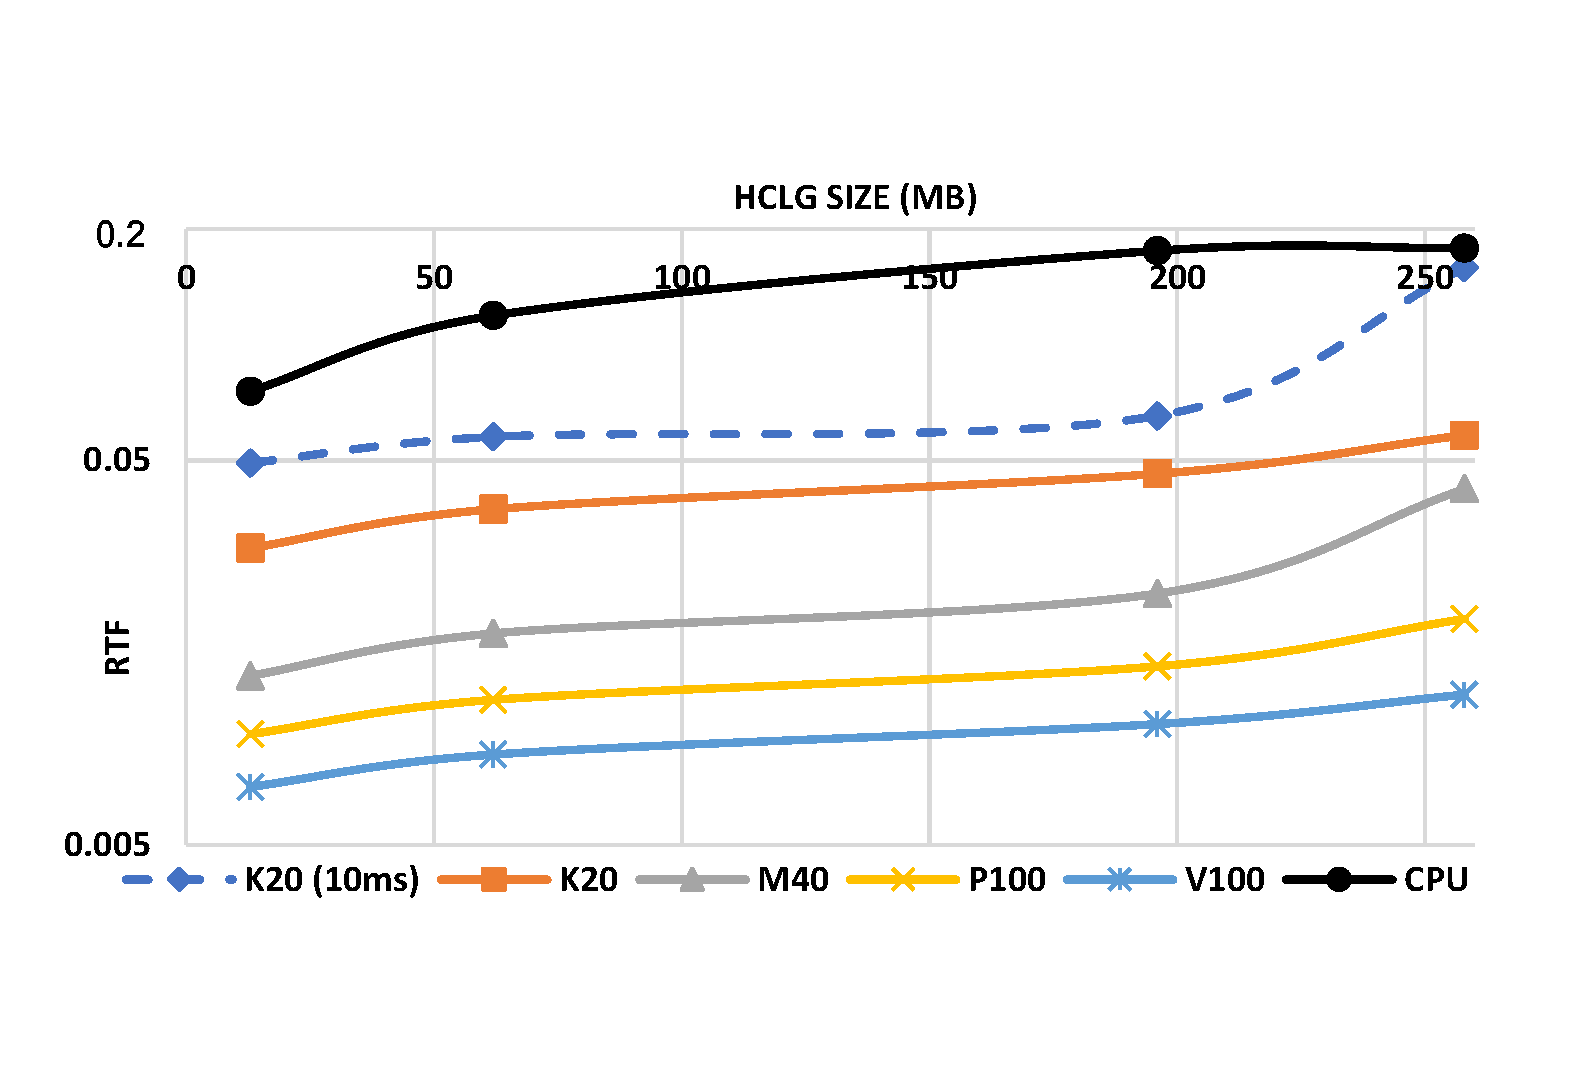
\includegraphics[width=\linewidth]{figure/gpu_analysis.pdf}
    \caption{\it  语言模型大小,帧率,GPU架构的比较}
    \label{fig:exp-ana}
\end{figure}

\begin{itemize} 
   \item Profiling.
   \vspace{-0.25em}
 \end{itemize} 
  图~\ref{fig:exp-profile} 比较了CPU和GPU的各个子模块的时间占用~\footnote{词图生成在CPU中被包含到令牌传递部分中} 。
  % (we can change this one to a histogram figure like this "Exploring Recognition Network Representations for Efficient Speech Inference.pdf", figure 4)
  GPU在显著快于CPU版本的同时,每部分分布比较均衡,显示出系统并没有显著的瓶颈。GPU解码器的令牌传递和词图处理都得到了显著加速。同时 ``other'' 部分包含了GPU的内核启动时间和同步等待时间。对于这些部分的优化也是未来研究的一个有意义话题。

\begin{figure}[ht]
  \centering
    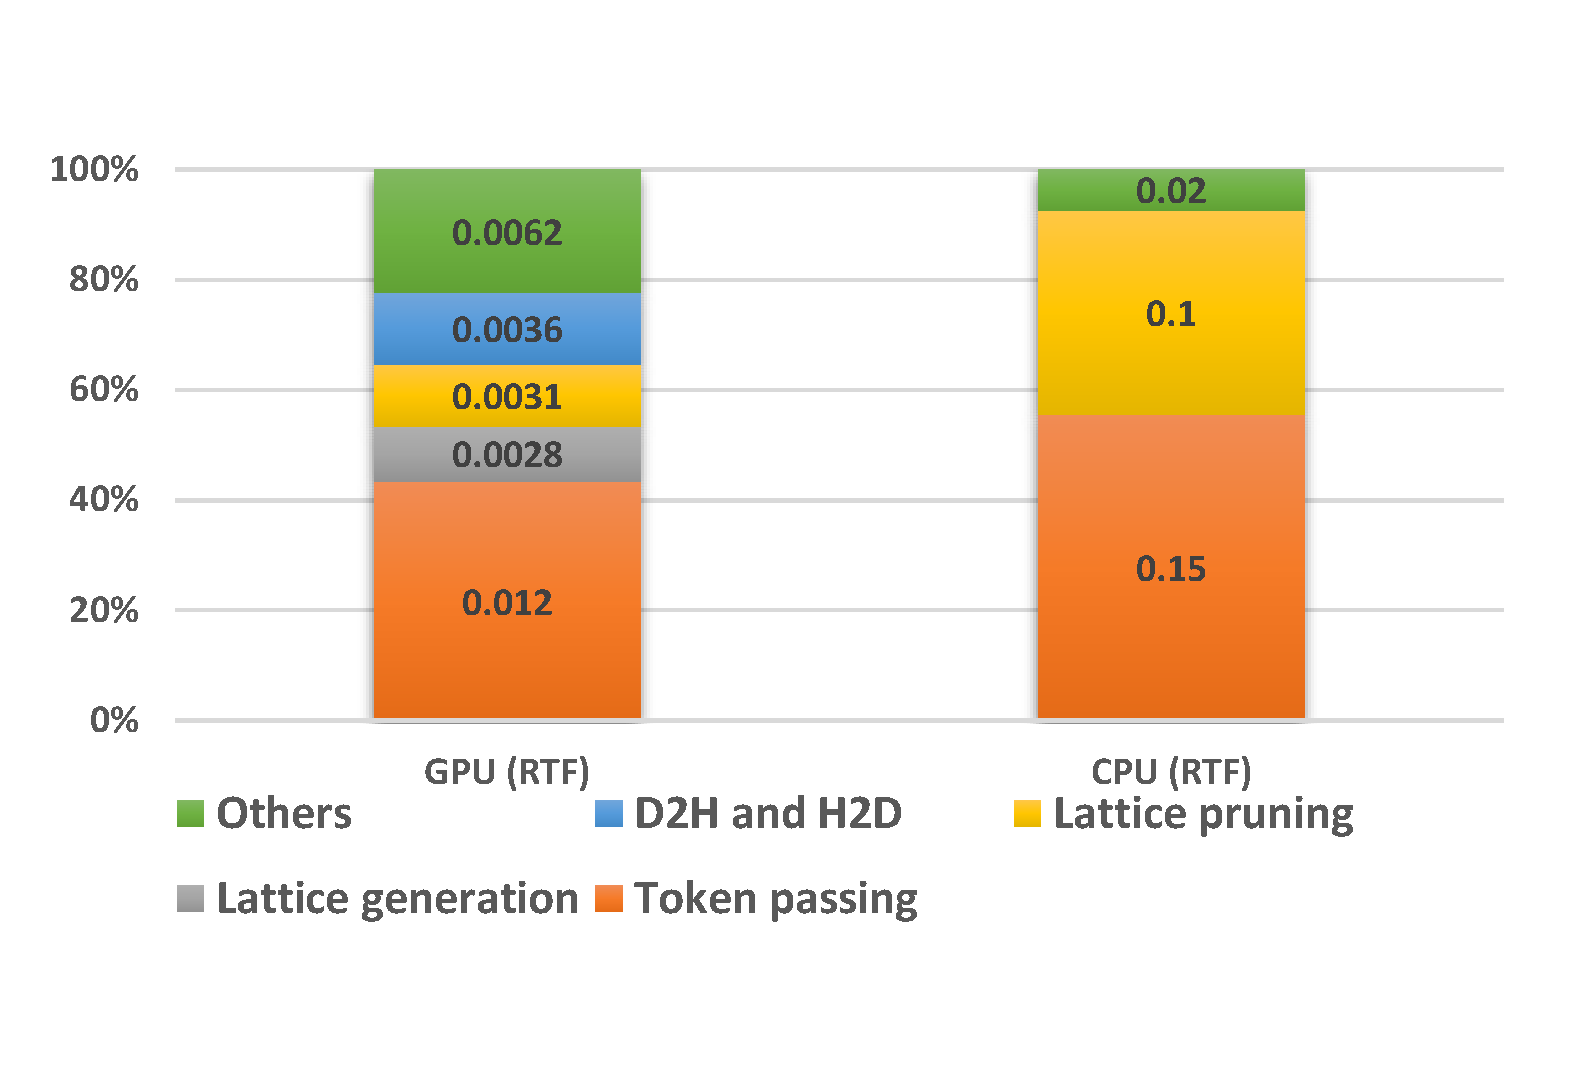
\includegraphics[width=1\linewidth]{figure/gpu_profile.pdf}
    \caption{{\it 针对解码器的时间占比分析} }
    \label{fig:exp-profile}
\end{figure}



\section{本章小结}
\label{chap:gpu-sum}

在这项工作中,我们描述了所提出的基于GPU并行计算的WFST解码器,我们将该实现融合在Kaldi开源工具包中。我们设计了并行版本的解码和词图处理算法。该系统相比CPU版本取得了显著的性能提升,并且该实现可以推广到大部分GPU架构中。最后,我们还将该实现完全开源。
